\section{Implementation}
\label{ch:intro:implementation}
% why basal ganglia
% (maybe first the anatomy)
The renowned neuroscientist, David Marr (1945--1980), proposed three levels of analysis to understand a complex system.
First, the \emph{computational level}, describes the task and the goal that need be achieved.
Second, the \emph{algorithmic level}, specifies the procedures for manipulating the information associated with the computation.
Third, the \emph{implementation level}, characterizes how to physically realize the algorithm~\cite{Willshaw2015Marr}.
\Citeauthor{Krakauer2017Neuron} in a perspective article that greatly influenced this work, present the following example~\cite{Krakauer2017Neuron}.
Understanding a flying bird could be achieved at three levels:
A bird attempts to \textit{fly} (level~1:~computation) by \textit{flapping} its wings (level~2:~algorithm) which is plausible due to aerodynamic properties of the \textit{feathers} (level~3:~implementation).
They then argue that the explanatory power of studying feathers alone is fundamentally restricted, evident by some birds that fly without feathers and some types of flight that does not require flapping.
As it pertains to the link between brain and behavior, it may be much more difficult to infer the algorithms used by brain from studying the nervous system, compared to understanding them at a computational level.
\par
Thus far, I portrayed the case for behavioral importance of time estimation (level~1), and different possible strategies to estimate an interval (dedicated, emergent, and embodied clock, level~2).
In this section, I will address how those strategies could be implemented in the brain (level~3).
Of all the brain regions that have been suggested to be involved in time perception\footnotemark, across a wide range of tasks and scales, \gls{bg} is of unique interest.
\footnotetext{
    So many brain structures have been found implicated in time estimation that prompted \citeauthor{Wittmann2013NatRevNeurosci} to state: ``one may be inclined to state that researchers are actually clueless concerning the question of how the brain processes time."~\cite{Wittmann2013NatRevNeurosci}.
    }
For decades, \gls{bg} have been the focus of many timing studies~\cite[see][]{Paton2018NeuronRev}, as well as motor studies~\cite[see][]{Turner2010CurrOpinNeurobiol}.
Therefore, it could be considered as an ideal candidate structure to mediate timing behavior through sensorimotor mechanisms.

%===========================================================
\subsection{The Basal Ganglia}
\label{intro:BGAnatomy}
The \glsentrylong{bg} are a set of interconnected subcortical nuclei.
Their neural organization, cell types, and neurochemical markers are highly conserved in vertebrates for over 500 million years, ranging from the lamprey to the primates~\cite{Grillner2016BG}.
The \gls{bg} may be viewed as a two-input two-output system.
The striatum and the \gls{stn} are the input structures receiving excitatory afferents from virtually the entire cerebral cortex and thalamus.
In rats, compared to \gls{stn}, the striatum contains more than two-hundred times more neurons and thus is regarded as the main input to the \gls{bg}~\cite{Oorschot1996}.
\par
The output nuclei are the internal segment of the globus pallidus, i.e., \gls{gpi}, and the \gls{snr}.
They are exclusively composed of GABAergic projection neurons with high baseline firing rates and target premotor centers in the brainstem and thalamus.
There are no direct connections from the \gls{bg} efferents to motor neurons of the brainstem or spinal cord~\cite{Mink1996}.
\par
Other than the input and output nuclei, the \gls{bg} also include the external segment of the globus pallidus, i.e., \gls{gpe}, which is innervated by the striatum and the \gls{stn}.
Most neurons in the \gls{gpe} provide GABAergic projection to the \gls{stn}, \gls{gpi}, and \gls{snr}~\cite{Dudman2015Book}.
The other nuclei of the \gls{bg} are the \gls{da}-containing centers of the midbrain, namely ventral tegmental area, and \gls{snc}.
These nuclei innervate striatal neurons in a dense and rather uniform manner, however, they also target structures external to the \gls{bg}, like several cortical and limbic regions.
\autoref{fig:intro:BGAnatomy} summarizes the anatomy of the \gls{bg}.

\begin{figure}[bth]
	\begin{center}
		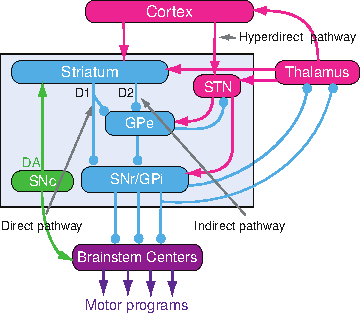
\includegraphics[width=0.7\linewidth]{ch-intro/figures/BGAnatomy}
		\caption[Anatomy of the Basal Ganglia]
		{\textbf{Schematic Anatomy of the basal ganglia.}
		The gray highlighted rectangle depicts the BG nuclei.
		Arrows show anatomical connections (\textit{red}: glutamatergic; \textit{blue}: GABAergic; \textit{green}: DAergic).
		STN:~subthalamic nucleus;
		GPe:~globus pallidus externus;
		SNc:~substantia nigra pars compacta;
		SNr:~substantia nigra pars reticulata;
		GPi:~globus pallidus internus;
		DA:~dopamine.
		Figure slightly modified from~\cite{Grillner2016BG}.
		}
		\label{fig:intro:BGAnatomy}
	\end{center}
\end{figure}

\subsubsection{Striatum} \label{intro:anatomy:striatum}
%order of material: MSNs > interneurons > I/O > D/ID pathway > dopamine > topography > DLS/DMS
The striatum is the main input nucleus of the \gls{bg} and one of the largest undivided structures in rodent brain atlas~\cite{Hintiryan2016NN}.
Despite having several cell types, GABAergic \glspl{msn} constitute~90--95\% of its neural population.
Their name stems from their morphological appearance, their size and the abundance of their dendritic processes~\cite{TURNER2000BasalFunction}.
\Glspl{msn} receive excitatory inputs from the cortex, thalamus, and amygdala.
Several other inputs modulate the responsiveness of the \glspl{msn} to massive excitatory synapses, namely \gls{da} afferents, inhibitory input from GABAergic interneurons (and from \gls{msn} collaterals), and input from cholinergic interneurons~\cite{Dudman2015Book}.
Consequently, \glspl{msn} are mostly quiescent, except during motor activity or in response to sensory stimuli~\cite{KandelBook2001}.
\par
Based on morphological and neurochemical identification, there are two major types of interneurons within the striatum, which make up~5--10\% of striatal neural population:
    the medium aspiny GABAergic interneurons, and the large aspiny cholinergic interneurons.
The most abundant type of GABAergic interneuron expresses parvalbumin.
Parvalbumin-positive interneurons are physiologically characterized by their hyperpolarized resting potential and fast spiking activity.
Thus, they are usually referred to as the \Glspl{fsi}~\cite{Dudman2015Book}.
They target \glspl{msn} at the soma level by gap junctions and provide powerful GABAergic synapses to several hundreds of surrounding \glspl{msn}~\cite{Grillner2016BG, Gage2010FSI}.
Although they are scarce, with higher firing rate compared to \glspl{msn}, they are capable of delaying action potentials in the neighboring \glspl{msn}~\cite{Wilson2007GABAergicNeostriatum}.
\par
Large cholinergic interneurons are the other type of striatal interneurons.
Their soma could be as large as~40~$\mu m$ in diameter, with expansive arborization and an axon that extends over~2~mm~\cite{Dudman2015Book}.
They have tonic discharge patterns, and in primate, are called \textit{tonically active neurons}.
\Glspl{fsi} and cholinergic interneurons are not noticeable in number, nonetheless, they are believed to strongly contribute to the dominance of inhibition in the striatum~\cite{Gage2010FSI}.
In addition to these two, several other types of interneurons within the striatum are described as well~\cite[see][]{Grillner2016BG, Dudman2015Book}.
\par
Massive excitatory projections from all areas of cortex target striatal \glspl{fsi} as well as \glspl{msn}.
Intralaminar nuclei of the thalamus also provide excitatory input (\autoref{fig:intro:BGAnatomy}).
Altogether, these glutamatergic synapses make up 80\% of all synapses in the striatum~\cite{Wilson2007GABAergicNeostriatum}.
Moreover, \gls{da}ergic afferents from the \gls{snc} are the main source of neuromodulatory influence.
They primarily synapse with principle neurons (\glspl{msn}).
\Gls{da} release modulates \gls{msn} activity differentially.
\par
\Glsentrylongpl{msn} are the only way out of the striatum.
They project to the globus pallidus and substantia nigra.
Based on their neurochemistry and projection patterns, they are divided into two distinct types.
One class expresses \glspl{d1} and projects directly to \gls{gpi}/\gls{snr} neurons, hence they form the so-called~\emph{direct pathway}.
The second kind expresses \glspl{d2} and projects to \gls{gpe}.
This path, in turn, leads to the output nuclei through two routes:~monosynaptic~\gls{gpe}$\rightarrow$output, or bisynaptic~\gls{gpe}$\rightarrow$\gls{stn}$\rightarrow$output projections~\cite{TURNER2000BasalFunction}.
These \glspl{msn} form the \emph{indirect pathway} (\autoref{fig:intro:BGAnatomy}).
Of note, \gls{stn} efferents form the only intrinsic excitatory connections in the basal ganglia, an otherwise inhibition-dominated structure.
\par
\Gls{da} significantly modulates neuronal activity in the striatum.
Axons from \gls{snc} neurons arborize widely in the striatum.
They mainly target the narrow necks connecting the spines to dendritic shafts, whereas cortical inputs mostly terminate on dendritic shafts.
This particular arrangement may be a mechanism by which \gls{da} release modulates cortical input to the \glspl{msn}~\cite{TURNER2000BasalFunction}.


\subsection{Basal Ganglia as a Clock}
\label{ch:intro:BGTime}

Many brain structures have been proposed to contribute to time estimation.
Among them, the \gls{bg}, are especially of interest, since they are directly involved in motor processes as well~\cite{Grillner2015}.
Moreover, the \gls{bg} are also involved in reinforcement learning---selecting actions in an uncertain world in a way that maximizes reward in the long term~\cite{Petter2018}.
Such learning necessitates an understanding of temporal contingencies in order to maximize future rewards.
Moreover, behavioral data supports that animals build probabilistic models for timing~\cite{li2013PNAS}.
% In general, execution of any complex behavior requires proper timing of the comprising sub-actions.
\par
The \gls{bg} are often implicated in timescales of several hundreds of milliseconds to several seconds~\cite{Paton2018NeuronRev}.
Evidence of involvement of the \gls{bg} in timing stems from a variety of sources, including pathologies such as \gls{pd}, lesion studies, and pharmacological and genetic manipulations.
\par
Following the taxonomy discussed in \autoref{ch:intro:taxonomy}, there is some evidence of involvement of the \gls{bg} in sensory timing.
\Citeauthor*{Rao2001} reported encoding of time intervals in the human striatum in a task in which subjects reported whether an interval were shorter or longer than a standard interval of 1200~ms.\footnotemark\
They also observed a dynamic network of cortical activity in inferior parietal, premotor, and dorsolateral prefrontal cortex.
These nodes in the network were attributed to different components of temporal processing, respectively, attention, memory, and interval comparison.
They collectively concluded implication of the ``striatal dopaminergic neurotransmission in hypothetical internal timekeeping mechanisms"~\cite{Rao2001}.
\footnotetext{
    This paradigm is commonly referred to as ``interval categorization task".
    }
Moreover, \Citeauthor*{Pouthas2005} investigated interval categorization for two durations (450~ms and 1300~ms).
They observed ramping striatal activity during both intervals.
They concluded a direct role of the basal ganglia in duration estimation, and that the caudate nucleus ``may support a clock mechanism"~\cite{Pouthas2005}.
Similar evidence exist in other species too.
\Citeauthor*{Gouvea2015Elife} trained rats in a sensory categorization task to judge whether an interval is shorter or longer than 1.5~s.
They decoded animals' choice and elapsed time from ensembles of striatal neuronal activity, whereas apparent behavior in an overhead video failed to do so.
Transient inactivation of the \gls{ds} impaired performance, however, it did not cause a systematic under-- or over--estimation~\cite{Gouvea2015Elife}.
\par
Furthermore, the \gls{bg} are also well studied for their role in motor timing.
\Citeauthor*{Matell2003} trained rats to receive a reward in a fixed interval reinforcement schedule.\footnotemark\
The interval alternated between 10~s (25\% of trials) and 40~s (75\% of trials).
After learning, animals increased their lever press rate around the reinforced intervals.
Electrophysiological recordings from the striatum showed neurons with tuned firing rate only around 10~s interval, but not 40~s, while apparent behavior of the animals is similar.
The authors then suggest that a population of duration-coding cells, each tune to different values, could accurately represent the elapsed time~\cite{Matell2003}.
\footnotetext{
    In operant conditioning, fixed interval reinforcement schedule refers to a type of conditioning whereby a response is reinforced only if a certain period of time has elapsed.
    }
\Citeauthor*{Mello2015} also used a similar task for intervals ranging between 12~s to 60~s.
They found striatal cells that rescaled their activity when intervals changed.
As rats adjusted to the new interval, time estimations decoded form population dynamics predicted animals' timing performance.
In another study, \Citeauthor*{Bakhurin2017JNeuro} used a conditioning paradigm to signal delayed reward delivery (2.5~s after cue onset).
Individual neurons recorded in the striatum and orbitofrontal cortex displayed sequential activity during the interval.
A machine learning algorithm was then trained to decode the elapsed time from the stimulus onset.
They showed that both striatal and cortical networks ``encoded time, but the striatal network outperformed the orbitofrontal cortex".
Interestingly, removing the neurons modulated by licking activity from the decoder significantly reduced its performance, however, it still remained higher than chance level~\cite{Bakhurin2017JNeuro}.
\par
Another source of impact in the \glsentrylong{bg} is the neuromodulatory effect of \gls{da}.
\Glsentrylong{da}'s role in reward processing and circuit dynamics of the striatum is discussed in \autoref{intro:BGAnatomy} and \autoref{intro:BGMotor}.
\Gls{da} is also believed to be involved in timing~\cite{Paton2018NeuronRev}.
In a peak interval procedure\footnotemark, \Citeauthor*{DeCorte2019} found that \gls{d2} blockade delayed start and stop times for an interval of 6~s.
Whereas, blockade of \glspl{d1} delayed stop times only.
Then they stressed the role of the \gls{ds} in timing, with \gls{da} ``being particularly critical for the temporal control of action"~\cite{DeCorte2019}.
\footnotetext{
    Peak interval procedure is a common task used to study timing.
    Similar to fixed interval schedules, a cue indicates that a response will be reinforced only after a certain period of time has elapsed.
    The profile of the response around the interval is then studied.
    }
\Glsentrylong{da} neurons encode reward prediction errors which requires accurate reward predictions~\cite[see][]{Berke2018NN}.
\Citeauthor*{Takahashi2016} recorded from \gls{da} neurons of rats while they performed a task with uncertainty in reward timing and reward number.
Neuronal activity showed error signals in response to both types of prediction error, however, after ventral striatal lesions, neurons only responded to changes in reward number, and not reward timing.
These results suggested that time-dependant component of reward prediction of \gls{da} neurons might rely on the ventral striatum~\cite{Takahashi2016}.
In an interesting study, \Citeauthor*{Paton2016Sci} measured and manipulated the activity of \gls{da} neurons in a 1.5~s interval categorization task.
\Gls{da}ergic activity predicted animal's time estimates.
Transient activation/inhibition of \gls{da} neurons caused under--/over--estimation of the interval.
Hence, they concluded that ``\gls{da} neurons, which are so central to reward processing, exert control over time estimation"~\cite{Paton2016Sci}, although these results reflect \gls{da} function in general, not specifically in the \gls{bg}.
Similar to scaling of neuronal activity in the striatum~\cite{Mello2015}, \gls{da} concentration in the \gls{ds} is also scalable to time intervals in several second time range~\cite{Howard2017}.
However, \citeauthor{Howard2017} then conducted a series of experiments and concluded that the \gls{da} signal in the \gls{ds} does not reflect interval timing per~se, rather it is specific to behavioral choice of action~\cite{Howard2017}.
\par
Deficits in temporal perception occur in many disorders.
Since pathologies usually affect multiple brain structures or manifest in several behavioral domains, it is unclear whether timing deficits are responsible for dysfunctions, or they are merely the result of other malfunctioning systems.
Schizophrenia, for example, is a complex psychiatric disorder with a wide range of symptoms, including: delusions, hallucinations, speech poverty, and timing deficits.
This impairment is reported in sensory and motor timing tasks and is associated with increased \gls{da} levels in the striatum, as well as abnormal activity in the dorsolateral prefrontal cortex and \gls{sma}~\cite[see][]{Snowden2019}.
Furthermore, it has been reported that individuals with attention deficit/hyperactivity disorder did not benefit from temporal predictabilities in an oculomotor task that displayed a target after a random delay~\cite{Dankner2017}.
Additionally, timing deficiency has also been reported in \gls{hd}.
Patients demonstrated lower sensitivity to temporal regularities and overall, poorer performance in different types of sensory timing tasks.
Their performance negatively correlated with the progression of the \gls{hd}~\cite{Cope2014}.
Finally, \gls{pd} also affects timing performance.
Lower timing performance has been reported in multiple tasks.
\Citeauthor*{Harrington1998} showed that \gls{pd} patients were impaired in sensory timing, in which `duration perception' was weaker compared to the control group.
Also, in a motor task, whereby subjects performed finger-tapping synchronized with a series of tones (in the subsecond range), \gls{pd} participants were significantly more variable~\cite{Harrington1998}.
Interestingly, it has been proposed that frequent exposure temporally-structured tones might alleviate motor symptoms of the \gls{pd}, especially gait and stride length~\cite{Dalla2017}.

\subsection{Basal Ganglia as a Sensorimotor System}
\label{intro:BGMotor}
\epigraph{Why do we and other animals have brains?\ldots You may reason that we have one to perceive the world or to think, and that is completely wrong\ldots We have a brain for one reason and one reason only, and that is to produce adaptable and complex movements.}
{\textit{Daniel Wolpert, TED talk}}
\noindent

Here, I am supposed to review the literature on the function of the \gls{bg}.

\subsubsection{Motor Control} \label{intro:motorControl}
\subsubsection{Motor Learning} \label{intro:motorLearning}
% \subsubsection{DLS}
% \subsubsection{DMS}
\subsubsection{Action Selection} \label{intro:actionSelection}
\subsubsection{Motor Habits} \label{intro:motorHabits}
\subsubsection{Cognition} \label{intro:bgCognition}
